%%%%%%%%%%%%%%%%%%%%%%%%%%%%%%%%%%%%%%%%%%%%%%%%%%%%%%%%%%%%%%%%%%%%
%%%%%%%%%%%%%%%%%%%%%%%%%%%%%%%%%%%%%%%%%%%%%%%%%%%%%%%%%%%%%%%%%%%%%
%%%%%%%%%%%%%%%%%%%%%%%%%%%%%%%%%%%%%%%%%%%%%%%%%%%%%%%%%%%%%%%%%%%%%
%%%%%%%%%%%%%%%%%%%%%%%%%%%%%%%%%%%%%%%%%%%%%%%%%%%%%%%%%%%%%%%%%%%%%

\chapter{Overview}

This document describes extensions and changes in \pml between versions 0.9 \& 0.8.1. 
The evolution of \pml since the project start are visualised in Figure \ref{fig:history}.

\begin{figure}[ht!]
\centering
  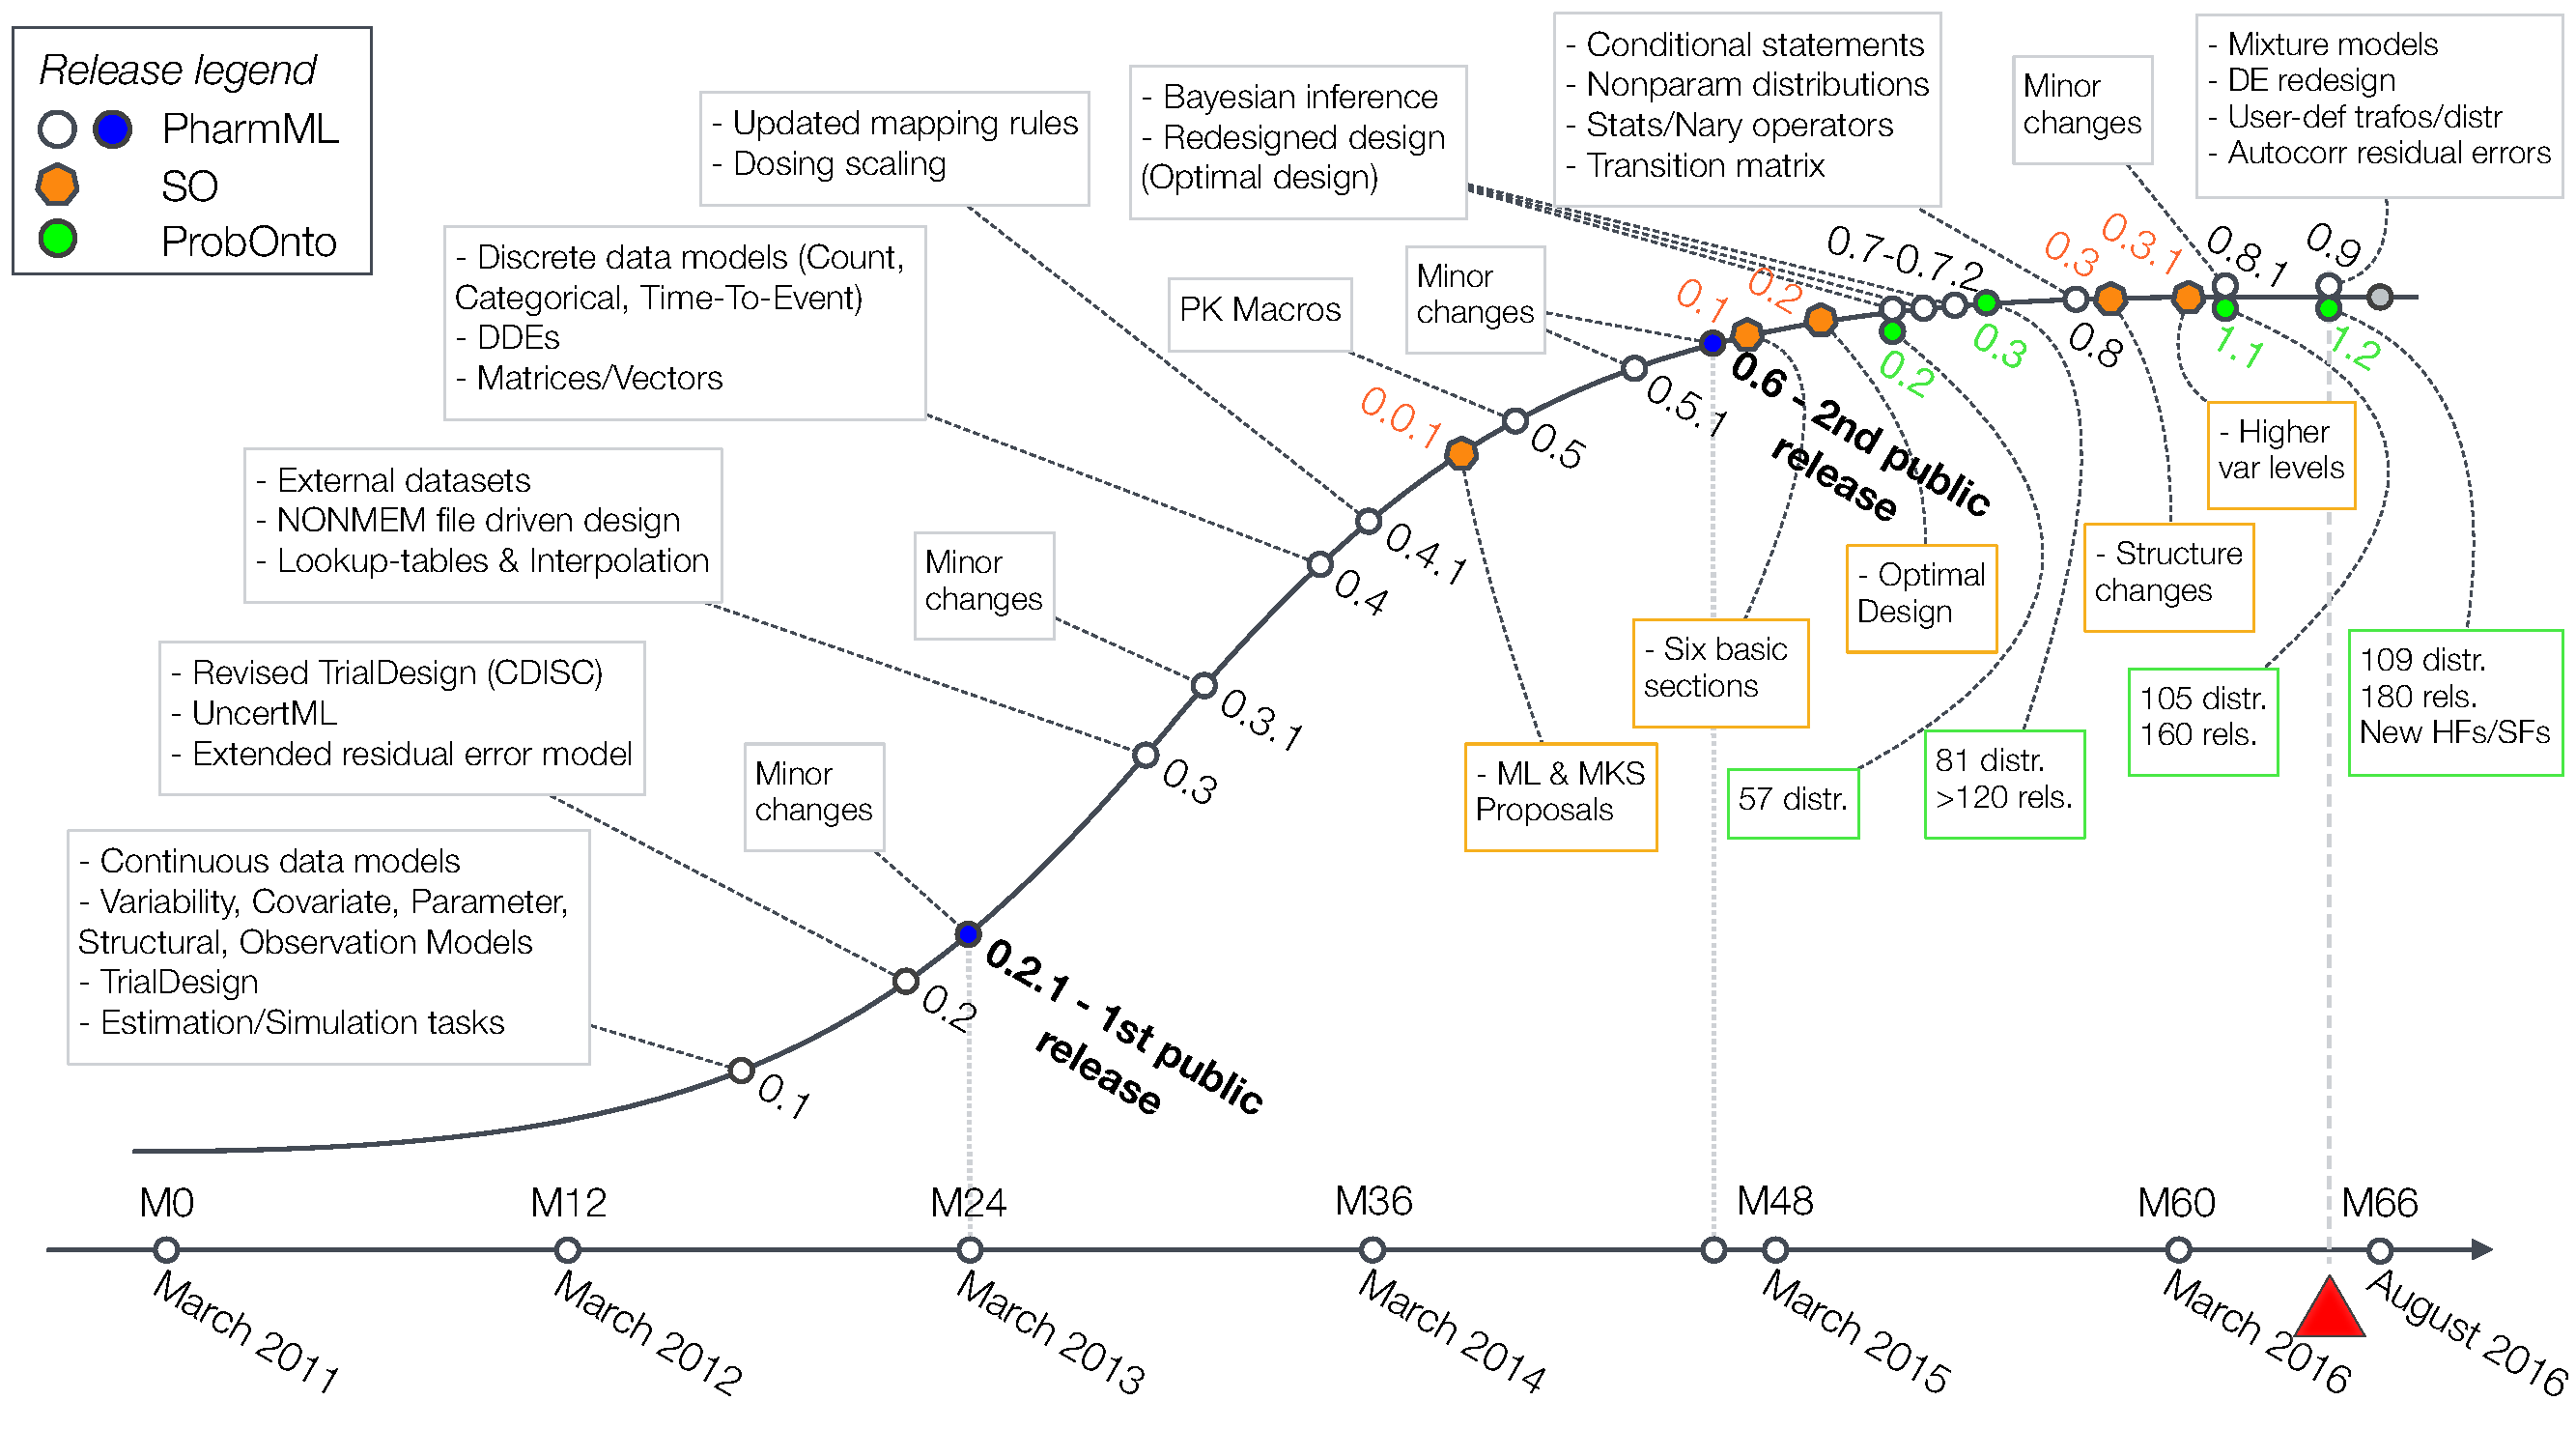
\includegraphics[width=160mm]{pics/Timeline-v09.pdf}
 \caption{PharmML/SO/ProbOnto release history with major extensions listed.}
 \label{fig:history}
\end{figure}

\section{Summary of changes/extensions in 0.9}
The following table summarises the major changes in version 0.9 compared to 0.8.1
described in detail in following chapters. 
	
\captionsetup[longtable]{skip=1em}
\LTcapwidth=\textwidth
\begin{center}
%\renewcommand{\arraystretch}{1.1}%
\begin{longtable}{lll}
\hline
\hline
\pml element 				&  version $\le$ 0.8.1 	& version 0.9 \\
or modelling aspect 			& 					& \\
\hline
\hline
  \multicolumn{3}{c}{\textit{General}}		\\
\hline
\hline
Box-Cox transformation		& standard  \xatt{BoxCox}  & {\color{red} \scshape{new}} \xatt{BoxCox2} version for negative values \\ 
Section \ref{sec:BoxCox2Trafo} &					& \\
\hline
User-defined transformations	& not supported 		& {\color{red} \scshape{new}} value \textit{userDefined} for attribute \xatt{type}  \\ 
Section \ref{sec:userDefTrafo} &					& \\
\hline
User-defined distributions		& not supported 		& {\color{red} \scshape{new}} \xelem{UserDefDistribution} element with  \\ 
Section \ref{sec:userDefDistros} &					& attribute \xatt{type} w. values CDF, PDF, HF, SF \\
\hline
Constants					&  			 		& imaginary unit $i$ added \\ 
Section \ref{sec:otherChanges}&					& \\
\hline
Vectors, Matrices			& 			 		& {\color{red} \scshape{new}} \xelem{EndIndex} element added \\
Section \ref{sec:EndIndex}	&					& \\
\hline
ODE initial values			& not supported  		& {\color{red} \scshape{new}} \xelem{InitialValue} element added \\
Section \ref{subsec:initialValue}&					& \\
\hline
Array dimension operator 	& not supported  		& {\color{red} \scshape{new}} \xelem{ArrayDim} element added with attribute\\
Section \ref{subsec:arrayDimOps}&					& \xatt{op} w. values \emph{length, ndims, numel, size} \\
\hline
ConditionalStatement		& different namespaces 	& one namespace \xatt{math:} only \\ 
\hline
\hline
  \multicolumn{3}{c}{\textit{Model Definition}}		\\
\hline
\hline
  \multicolumn{3}{c}{\textit{Covariate model}}		\\
\hline
Discrete covariates			& reference category  	& {\color{red} \scshape{new}} \xelem{referenceCategory} element  \\
Section \ref{subset:catCovTrans}& annotation not supported	& and the \textit{latent} value of the \xatt{type} attribute \\
\hline
Creating new categorical 		& not supported		& referencing possible via \xelem{CatRef} with   \\
covariates by clustering		& 					& additional \xatt{symbIdRef} and \xatt{blkIdRef} attribute \\
Section \ref{subset:catCovTrans} &					& \\
\hline
Latent covariates			& not supported 		& {\color{red} \scshape{new}} \xelem{NumberOfCategories} element  \\
Section \ref{subsec:latent}	& 					& and the \textit{latent} value of the \xatt{type} attribute \\
\hline
Exclusion/inclusion criteria	& not supported 		& {\color{red} \scshape{new}} \xelem{Criteria} element with \xatt{type} \\
Section \ref{subsec:exclInclCriteria}	&				& \emph{exclusive, inclusive} values  \\
%\hline
%  \multicolumn{3}{c}{\textit{Structural model}}		\\
%\hline
%ODEs					& ODE with DV &  \\
%Section \ref{sec:ODEreloaded}	& 						&  \\
%\hline
%PDEs					& not supported 			&  \\
%Section \ref{sec:PDEs}	& 	&  \\
\hline
Parameter model   			& not supported 			& Elements \xelem{RandomEffects}, \xelem{FixedEffect}, \\
Section \ref{subsec:symbRefAssign}	& 				& \xelem{RandomVariable1}, \xelem{RandomVariable2} \\
						&						& accept any expressions \\
\hline
  \multicolumn{3}{c}{\textit{Structural model}}		\\
\hline
%\xatt{curl} $\equiv \nabla \times $ -- curl operator
%%-- curl operator acts on a vector field, F, and represents the rotation at a point.
%\item 
%\xatt{divergence} $\equiv \nabla \cdot $  -- divergence operator
%%-- divergence measures the rate per unit volume at which the fluid (or other "stuff") is flowing away from the point
%\item 
%\xatt{gradient} $\equiv \nabla $  -- gradient operator
%%-- gives the magnitude and direction of the greatest rate of change of f
%\item 
%\xatt{laplacian}  $\equiv \nabla^2 $  -- laplace operator
Calculus operators 			& not supported 			& {\color{red} \scshape{new}} \xelem{VectorCalcOp} with \xatt{op} attribute \\
Section \ref{sec:CalcBuildingBlocks}	&					& values \emph{curl, divergence, gradient, laplacian}\\
\hline
ODEs, PDEs				& basic support				& {\color{red} \scshape{new}} \xelem{DE} element with child elements  \\
Chapter \ref{ch:DEs}		& 						&  \xelem{BoundaryCondition}, \xelem{Diff}, \xelem{DiffVariable} etc.\\ 
\hline
  \multicolumn{3}{c}{\textit{Observation model}}		\\
\hline
Mixture models   			& not supported  			& {\color{red} \scshape{new}} \xelem{MixtureModel} with child elements \\
Section \ref{sec:mixStructModels}	& 					& \xelem{Proportions}, \xelem{GroupLabel} and \\
						&						& \xelem{GroupProbabilities} and attributes \xatt{symbId}  \\
						&						& and \xatt{type} with values \{\textit{wsmm}, \textit{bsmmSupervised} \\
						&						& and \textit{bsmmUnsupervised}\}\\
\hline
Multiple models support 	  	& allowed only one  			& -- multiple observations per model supported \\
Section \ref{sec:obsModel}	& observation per block		& -- conditional declaration supported \\
\hline
Autocorrelation of residual  	& not supported			& {\color{red} \scshape{new}}  \xelem{Autocorrelation} tag with \xatt{type} \\
errors, Section \ref{subsec:autoCorr}	& 				&  attribute and child elements \xelem{TimeStepNo} \\
						&						& \xelem{CorrParameters} \\		
\hline
Section \ref{sec:obsModel}	& one observation per block	& multiple observations allowed \\
						& declaration only			&  \\
\hline
Discrete data  				& count data models named 	& removed \xelem{IntensityParameter}, \\
Section \ref{subsec:namedParams}	& parameters available	& \xelem{DispersionParameter} etc.\\
\hline
\hline
  \multicolumn{3}{c}{\textit{Trial Design}}		\\
\hline
\hline
Observations  				& missing elements 			& {\color{red} \scshape{new}} \xelem{DeltaTime}, \xelem{BQL}, \xelem{UQL} \\
Section \ref{subsec:DeltaTime}	& 						&  \\
\hline
Covariates declaration		& in top trial design level only	& permitted arm-wise as well \\
Section \ref{subsubsec:defCovariates} 	&				&  \\
\hline
Referencing covariates   		& referencing of covariates	& referencing of individual covariates and covariate \\
Section \ref{sec:covModel} 	& not supported			& models required with attribute and {\color{red} \scshape{new}} \\
						&						& \xelem{CovariatesReference} in modelling steps \\
\hline
Referencing occasions   		& not supported		 	& {\color{red} \scshape{new}} \xelem{OccasionListRef} element \\
Section \ref{subsec:declOccs} & 						&  \\
\hline
Design spaces  			& no \xatt{oid}'s			& -- mandatory \xelem{oid} attributes \\
Section \ref{subsec:designSpaceId}	& 					& -- referencing of design spaces in optimal  \\
						&						& design with {\color{red} \scshape{new}} \xelem{DesignSpaceReference} \\
\hline
Dataset column types   		& 						& {\color{red} \scshape{new}} \xatt{columnType} values \emph{DATE, DAT1} \\
Section \ref{subsec:dataSets} 	& 						& \emph{DAT2, DAT3, YTYPE} \\
\hline
\hline
  \multicolumn{3}{c}{\textit{Modelling steps}}		\\
\hline
\hline
Tool-specific settings		& not supported			& {\color{red} \scshape{new}} \xatt{tool} attribute in \xelem{Operation} \\
Section \ref{sec:modelSteps}	&						& 	\\
\hline
\hline
  \multicolumn{3}{c}{\textit{ProbOnto}}		\\
\hline
\hline
Parametric distributions 		& 						& {\color{red} \scshape{new}} distributions LogNormal7($\mu_N$, $\sigma_N$),  \\
\cite{ProbOnto:2016e} 		&						& Trapezoidal1($a, b, c, d$), HalfNormal2($\mu, \sigma$) \\		
						&						& and WienerDiffusionModel1($\alpha, \beta, \delta, \tau$) \\
\hline
Empirical distributions/ 		& supported but inconsistent 	& {\color{red} \scshape{new}} \xelem{Realisation}  and \xelem{Weight} elements \\
\cite{ProbOnto:2016e} 		& mapping				& for declaring and mapping with dataset  \\
%\hline
%\hline
%  \multicolumn{3}{c}{\textit{UncertML}}		\\
%\hline
%\hline
%Distributions encoding 		& 						& removed -- replaced by ProbOnto  \\	
\hline
\caption{Overview of major differences between versions 0.9 and 0.8.1}
\label{figTable:overviewTable}
\vspace{-2em}
\end{longtable}
\end{center}